\section{Создание инстанса в OpenStack} \label{pril:f}

Сервис TryStack\footnote{\url{https://trystack.openstack.org}} позволяет использовать готовое окружение OpenStack без развертывания сложной инфраструктуры на локальных серверах.

Для регистрации на сервисе TryStack необходимо иметь аккаунт в Facebook и вступить в группу TryStack\footnote{\url{https://www.facebook.com/groups/269238013145112}}.

После отправки заявки на вступление в закрытую группу, возможно, придется подождать несколько дней для подтверждения заявки.
Когда заявка подтверждена, то можно авторизоваться в панели\footnote{\url{https://x86.trystack.org/dashboard/auth/login/?next=/dashboard/}} TryStack с помощью аккаунта Facebook.

После авторизации можно посмотреть интерфейс управления OpenStack (рис.~\ref{pic:ui}).
\begin{figure}[ht]
    \centering
    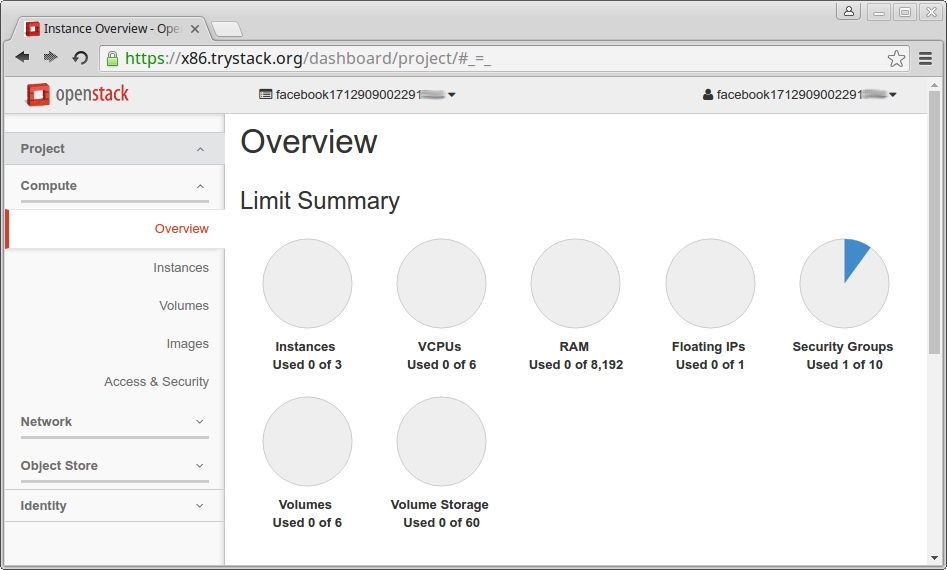
\includegraphics[width=\linewidth]{4_ui}
    \caption{Интерфейс управления OpenStack}\label{pic:ui}
\end{figure}

OpenStack позволяет создавать множество инстансов из готовых шаблонов ОС, также существует возможность создавать свои образы.
Доступные шаблоны ОС можно увидеть в разделе \textbf{Compute - Images}.

Для настройки OpenStack, в первую очередь, необходимо настроить сеть.

Создадим в разделе \textbf{Network - Networks - Create Network} (рис.~\ref{pic:net}):
\begin{itemize}
    \item внутреннюю сеть с именем student-net;
    \item подсеть student-subnet (192.168.0.0/24);
    \item укажем пул используемых IP-адресов (192.168.0.2 -- 192.168.0.10);
    \item и укажем DNS-сервера (8.8.8.8, 8.8.4.4).
\end{itemize}

\begin{figure}[ht]
    \centering
    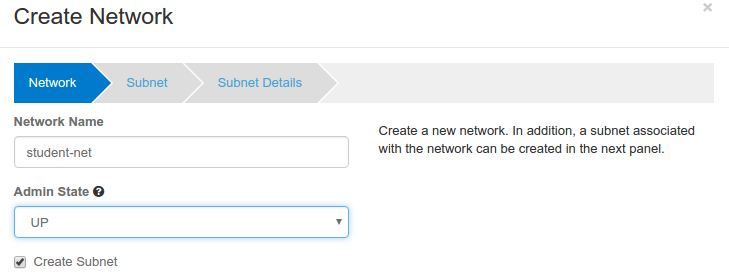
\includegraphics[width=0.9\linewidth]{6_net}
    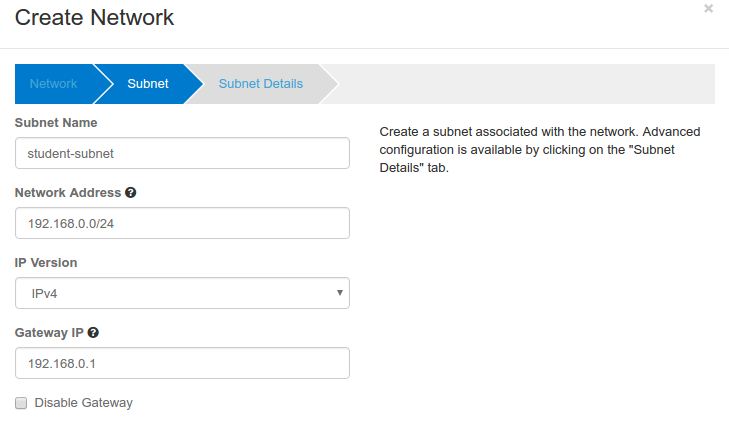
\includegraphics[width=0.9\linewidth]{7_net}
    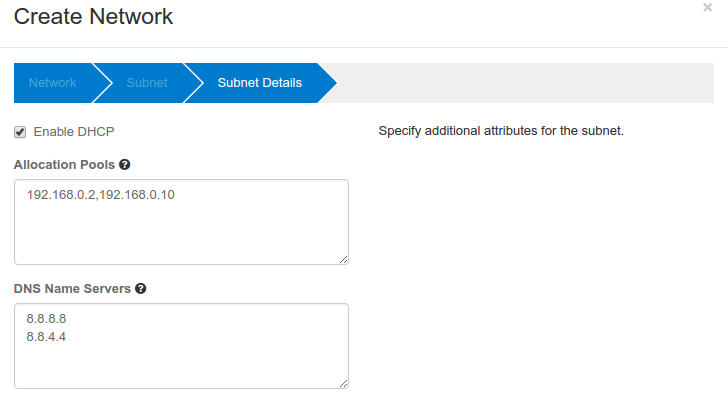
\includegraphics[width=0.9\linewidth]{8_net}
    \caption{Настройка внутренней сети}\label{pic:net}
\end{figure}

\clearpage

После создания внутренней сети, необходимо создать маршрутизатор, который соединит внешнюю сеть (public) с внутренней (student-net), сделать это можно в разделе \textbf{Network - Routers - Create Router} (рис.~\ref{pic:router}).
\begin{figure}[ht]
    \centering
    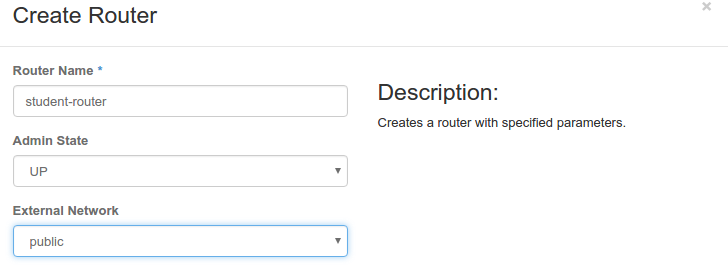
\includegraphics[width=\linewidth]{9_router}
    \caption{Создание маршрутизатора}\label{pic:router}
\end{figure}

Текущую топологию сети можно увидеть в разделе \textbf{Network - Network Topology} (рис.~\ref{pic:topology}).

На схеме видно, что маршрутизатор (student-router) связан с внешней сетью (public), но не с внутренней (student-net).
\begin{figure}[ht]
    \centering
    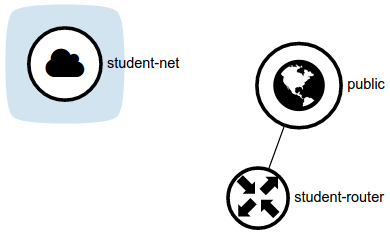
\includegraphics[width=0.5\linewidth]{10_topology}
    \caption{Текущая топология сети}\label{pic:topology}
\end{figure}

Соединяем маршрутизатор с внутренней сетью.
Щелкаем мышью на маршрутизатор и выбираем пункт \textbf{Add Interface}, добавляем внутреннюю сеть (student-net) к маршрутизатору, в качестве шлюза указываем адрес 192.168.0.1 (рис.~\ref{pic:addif}).
\begin{figure}[ht]
    \centering
    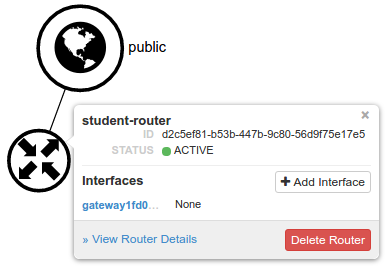
\includegraphics[width=0.5\linewidth]{11_addif}
    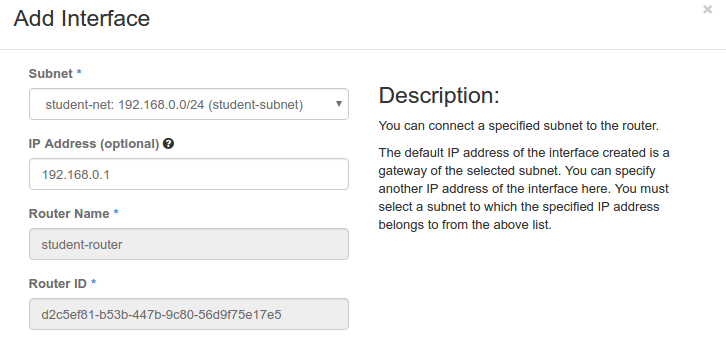
\includegraphics[width=\linewidth]{12_addif}
    \caption{Подключение внутренней сети к маршрутизатору}\label{pic:addif}
\end{figure}

После этого можно посмотреть на новую топологию сети (рис.~\ref{pic:new_topology}).
На этой топологии видно, что маршрутизатор соединяет внутреннюю и внешнюю сети.
\begin{figure}[ht]
    \centering
    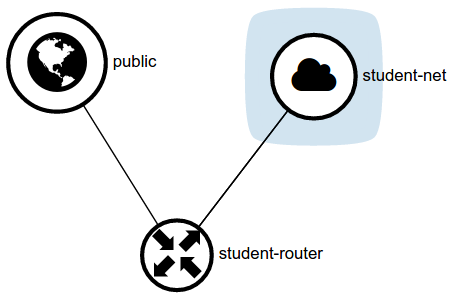
\includegraphics[width=0.5\linewidth]{13_newtopology}
    \caption{Маршрутизатор соединяет внешнюю и внутреннюю сети}\label{pic:new_topology}
\end{figure}

На этом настройка сети для OpenStack окончена.

\clearpage

По умолчанию для подключения к инстансам используется подключение по SSH с помощью шифрованых ключей.
Поэтому необходимо создать пару ключей, сделать это можно в разделе \textbf{Access \& Security - Key Pairs - Create Key Pair}.
Пусть это будет пара ключей с именем student123.

После создания пары ключей, автоматически скачается файл student123.pem, который нужно будет использовать для соединения к инстансам.

Для соединения к инстансу с внешнего мира, необходимо иметь выделенный внешний IP-адрес.
В TryStack можно получить только один такой адрес, сделать это можно в разделе \textbf{Compute - Access \& Security - Floating IPs - Allocate IP To Project}.
В некоторых случаях возможно, что выделить внешний IP-адрес не удается, в таком случае необходимо попробовать запросить адрес позже, предварительно обновив веб-страницу, это связано с ограниченным пулом IP-адресов, поэтому для всех пользователей TryStack таких адресов может не хватать.

После получения внешнего адреса, его можно увидеть в списке (рис.~\ref{pic:float_ip}).
\begin{figure}[ht]
    \centering
    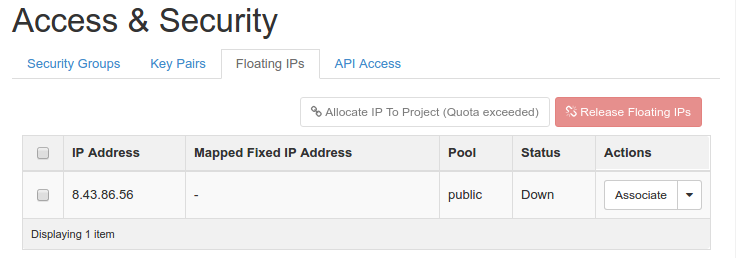
\includegraphics[width=\linewidth]{16_floatip}
    \caption{Список выделенных внешних IP-адресов}\label{pic:float_ip}
\end{figure}

Далее необходимо создать группу безопасности, в которой можно настроить правила фильтрации трафика для инстансов.
В разделе \textbf{Compute - Access \& Security - Security Groups - Create Security Group} создадим группу my-secgroup.

После создания группы, в общем списке выбираем пункт \textbf{Manage Rules} для my-secgroup.
Там можем видеть, что по умолчанию для данной группы открыты все исходящие соединения для IPv4 и IPv6.
Создадим разрешающее правило для входящих соединений по протоколу ICMP (рис.~\ref{pic:icmp}).
\begin{figure}[ht]
    \centering
    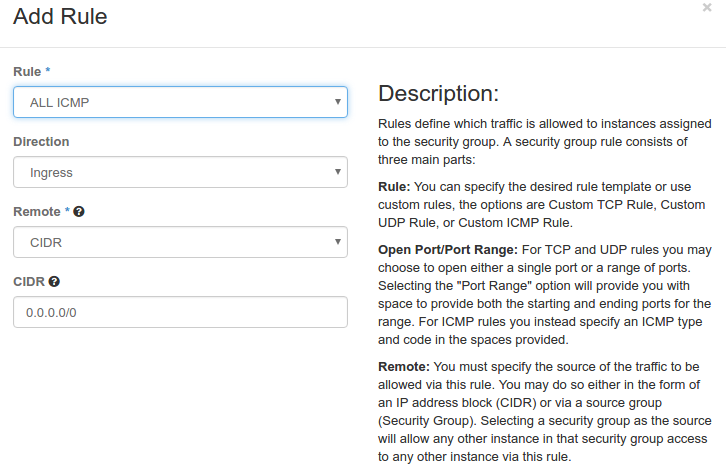
\includegraphics[width=\linewidth]{103_icmp}
    \caption{Разрешающее правило для работы ICMP}\label{pic:icmp}
\end{figure}

Аналогично создадим разрешающие правила для TCP и UDP (рис.~\ref{pic:rules}).
\begin{figure}[ht]
    \centering
    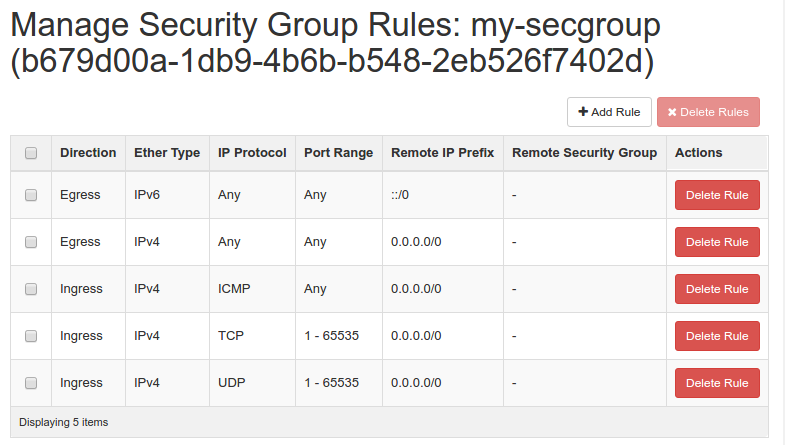
\includegraphics[width=\linewidth]{104_rules}
    \caption{Разрешающие правила для группы безопасности my-secgroup}\label{pic:rules}
\end{figure}

\clearpage

Далее мы можем создать первый инстанс (\textbf{Compute - Instances - Launch Instance - Details}).
Создадим его на базе ОС Ubuntu 16.04, размер инстанса m1.small (2048MB RAM, 20GB HDD).
Имя инстанса student-instance (рис.~\ref{pic:instance}).

В разделе \textbf{Access \& Security} укажем пару ключей student123 и группу безопасности my-secgroup.
В разделе \textbf{Networking} выберем сеть student-net.
\begin{figure}[ht]
    \centering
    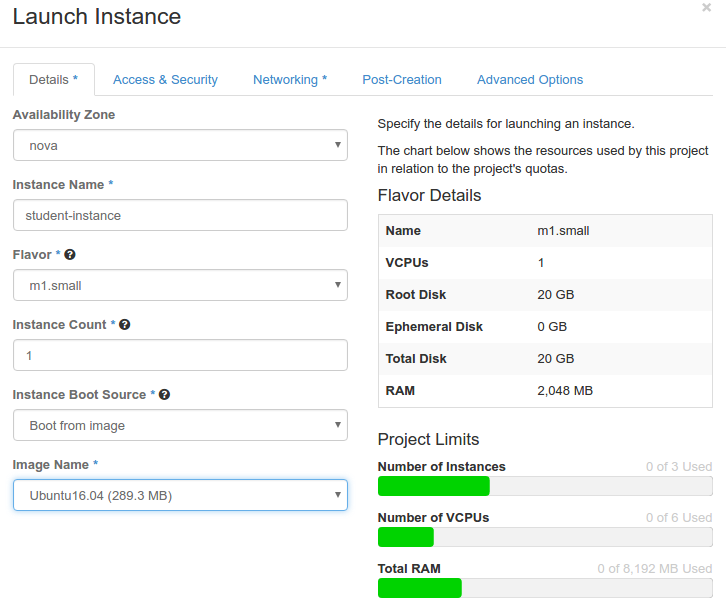
\includegraphics[width=0.8\linewidth]{17_instance}
    \caption{Создание нового инстанса}\label{pic:instance}
\end{figure}

После этого можно видеть запущенный инстанс в общем списке (рис.~\ref{pic:list}), ему присвоен внутренний адрес 192.168.0.3.
\begin{figure}[ht]
    \centering
    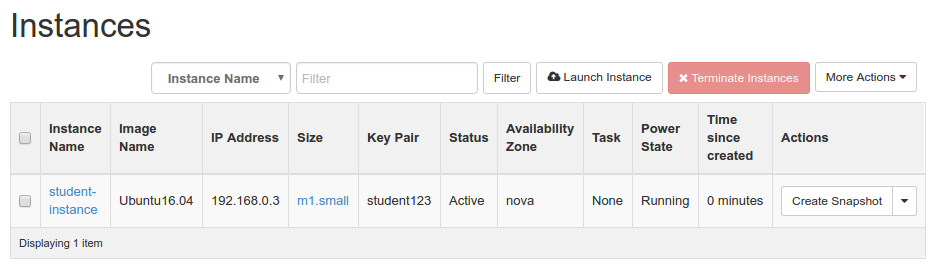
\includegraphics[width=\linewidth]{20_list}
    \caption{Список созданных инстансов}\label{pic:list}
\end{figure}

\clearpage

Для того, чтобы получить доступ к инстансу с внешней сети, необходимо привязать к инстансу внешний IP-адрес.
В разделе \textbf{Compute - Access \& Security - Floating IPs} напротив IP-адреса нажимаем кнопку \textbf{Associate}, затем указываем, что ассоциируем адрес с инстансом student-instance.

После этого в списке инстансов видим, что student-instance присвоен внешний IP-адрес 8.43.86.56 (рис.~\ref{pic:extip}).
\begin{figure}[ht]
    \centering
    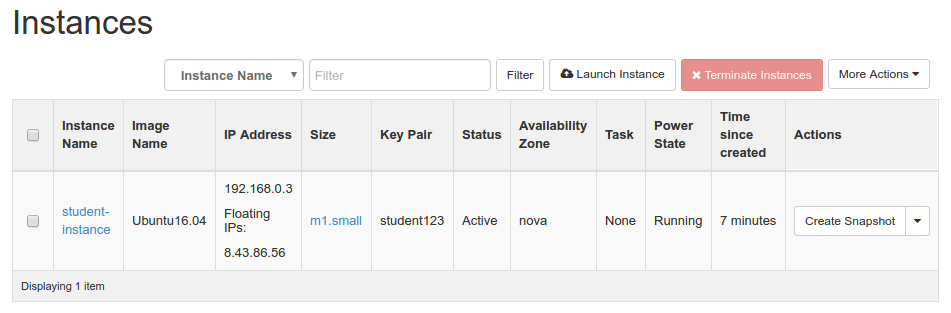
\includegraphics[width=\linewidth]{23_extip}
    \caption{Подключение внешнего IP-адреса к инстансу}\label{pic:extip}
\end{figure}

После того, как к инстансу привязан внешний адрес, можно проверить его доступность, соединившись по SSH:
\begin{lstlisting}
$ ssh ubuntu@8.43.86.56 -i Downloads/student123.pem
\end{lstlisting}

Инстансы созданные в TryStack доступны на протяжении 24 часов, так как сервис бесплатный, он позволяет только взглянуть на то, как работает OpenStack, поэтому он не годится для размещения своих проектов в облаке.

Установим для примера веб-сервер Nginx и разместим для общего доступа HTML-страничку.
\begin{lstlisting}
$ sudo apt update && sudo apt install nginx
$ sudo echo "<h1>Hello, this instance created by OpenStack.</h1>" > \
> /var/www/html/index.nginx-debian.html
$ sudo echo "<h3>Computer Science and Engineering, SevSU</h3>" >> \
> /var/www/html/index.nginx-debian.html
\end{lstlisting}

Заходим из веб-браузера по IP-адресу инстанса и видим результат работы веб-сервера (рис.~\ref{pic:html}).
\begin{figure}[ht]
    \centering
    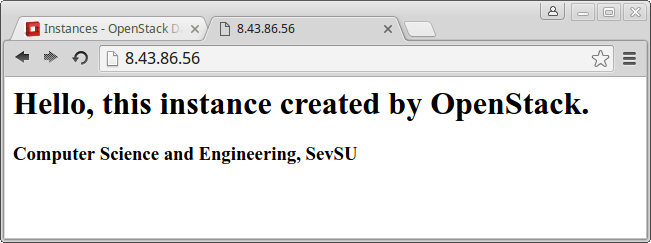
\includegraphics[width=0.8\linewidth]{24_html}
    \caption{Демонстрация работы веб-сервера в облаке}\label{pic:html}
\end{figure}

\clearpage
